O grupo 1 da disciplina de Projeto Integrador 1 do segundo semestre de 2015 deverá desenvolver um projeto de balão cativo para monitoramento do estacionamento e das fronteiras do campus da FGA, cujo objetivo é manter um maior controle da movimentação de carros e pessoas nas áreas de alcance do balão, devido os problemas de furtos avaliados anteriormente e, também, devido a possíveis invasões de área.

O estacionamento possui área de 16100 $m^2$, com perímetro de 1215 m. Contudo, a área é extensa e existem locais de estacionamento isolados [figura \ref{img:fga2}].

\begin{figure}[H]
  \centering
  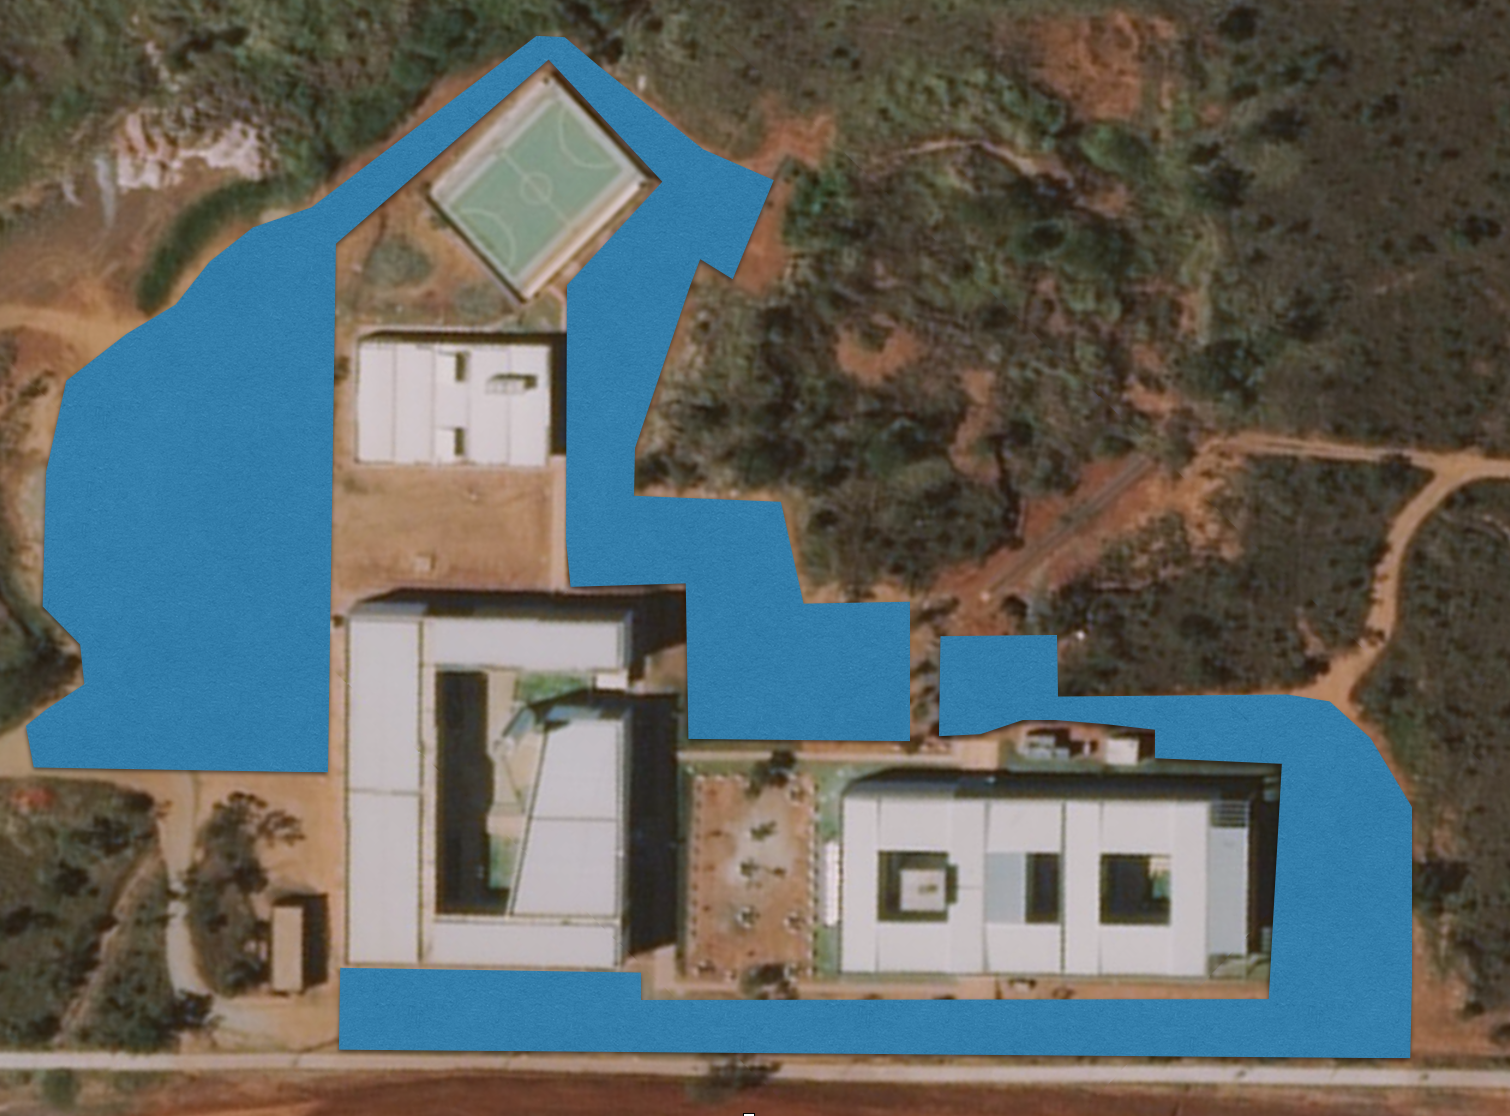
\includegraphics[width=0.87\textwidth]{figuras/fga2}
  \caption{Vista aérea do Campus FGA: áreas de estacionamento do campus.}
  \label{img:fga2}
\end{figure}

Dessa forma, devido à impossibilidade de localizar apenas um balão que possa monitorar todas as áreas de estacionamento, três balões cativos serão posicionados estrategicamente para que o objetivo seja cumprido [figura \ref{img:fga3}].

\begin{figure}[H]
  \centering
  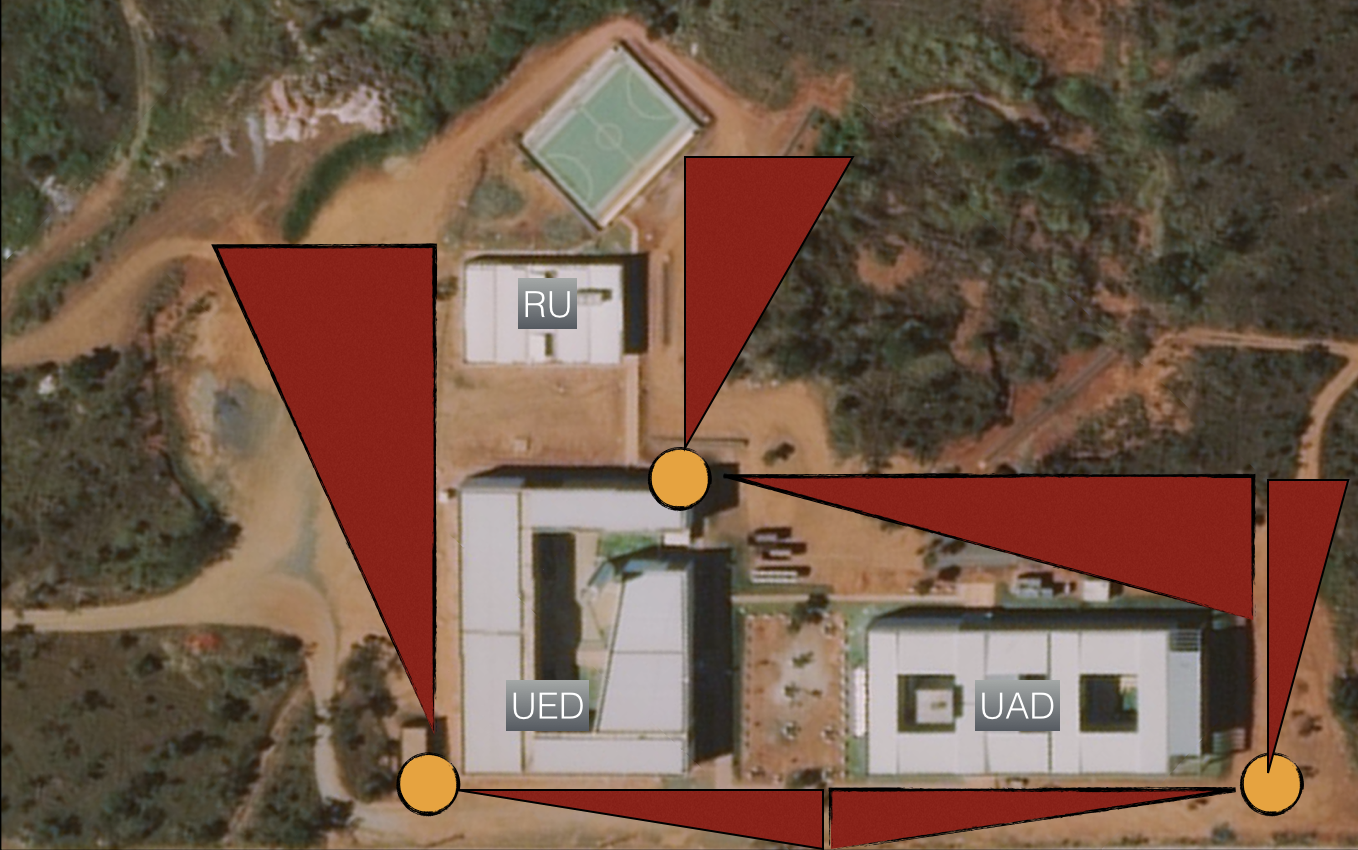
\includegraphics[width=0.87\textwidth]{figuras/fga3}
  \caption{Vista aérea do Campus FGA: áreas de alcance de monitoramento.}
  \label{img:fga3}
\end{figure}

\section{Estrutura e Funcionamento}
  A estrutura do balão será dividida em três partes principais: a bexiga, local onde será armazenado o gás; payload, que será o local de armazenamento dos equipamentos eletrônicos; elevador, que consite o cabo preso à payload do balão e também o sistema eletromecânico em solo que libera o fio (elevando o balão) ou retrai o fio (desce o balão).

  \subsection{Payload}
    A estrutura da payload foi inspirada em um padrão de nanosatélites 9U, figura \ref{img:payload}, porém com adaptações. A estrutura de um CubeSat 1U possui as dimensões deste são de um cubo 10 x 10 x 10 cm, ou seja, o termo 1U diz respeito as dimensões do sistema. Dessa forma um 9U significa que suas dimensões são 30 x 30 x 10 cm, e colocando de outra forma, é equivalente à três nanosatélites 3U em conjunto. A parte superior será acoplada à bexiga, enquanto que a inferior, ao cabo.

    \begin{figure}[H]
      \centering
      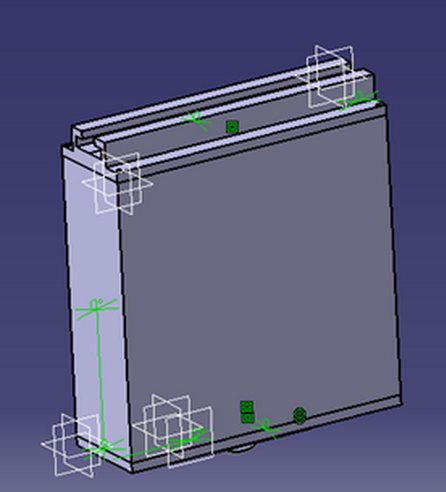
\includegraphics[width=0.5\textwidth]{figuras/payload}
      \caption{Representação da estrutura da payload. }
      \label{img:payload}
    \end{figure}

  \subsection{Balão}
    Segundo Yajima, existem três tipos de sistemas de balões que são utilizados: balão zero pressão, balão super-pressão e uma combinação entre os dois sistemas. O sistema mais adequado à aplicação proposta mostrou-se o balão zero pressão.Existem vários modelos de balão: esférico, cilíndrico, tetraédrico e formato natural. O modelo utilizado será o modelo de balão esférico, pois esse modelo é o que apresenta menos complicações nos cálculos de dimensionamento de volume, empuxo, gás e etc.

  \subsection{Gás}
    O gás que será utilizado no balão será o Hélio, este gás possui algumas desvantagens em relação ao gás Hidrogênio[2], que é mais leve, porém por ser um gás inerte o Hélio é a principal opção  de uso[3]. Ficou decidido que a massa  máxima  da payload será de 20 kg.

  \subsection{Material}
    O material usado para a confecção da bexiga será a Aramida (Kevlar), pois  esse material apresenta propriedades mecânicas interessantes, como elevada tenacidade, baixo alongamento e resistência ao calor[10],  além de ser considerado um material leve[8]. Com esses dados em mãos foi possível calcular o raio mínimo que o balão deveria ter, o valor foi de 2 metros. Para uma margem de segurança será adotado um valor de raio do balão entre 2 metros e 2,5 metros. As forças de empuxo e peso do balão variam de acordo com o raio. O empuxo com o raio igual a 2 metros é de cerca de 403N, com o raio igual a 2,5 metros o empuxo é de 786N, será avaliado o material utilizado na ancoragem do balão,  e dependendo da resistencia à tração desse material será adotado um raio fixo para o balão.

  \subsection{Funcionamento}
    O horário de funcionamento do balão será das 6h às 21h, o sistema ficará a uma altura entre 30 metros e 50 metros para uma melhor visualização do movimento do estacionamento.

    O estudo das condições ambientais e o dimensionamento dessas variáveis são fundamentais para a estabilidade do balão. A força de arrasto no balão devido a um vento de 12m/s, na pior das hióteses, seria na ordem de 3,8kN.
